% Copyright 2026 Sreeram Anil
% SPDX-License-Identifier: CC-BY-4.0
% =============================================================================
%  Decentralised pack filtering with a sigma-point cell filter — pack-level family
% =============================================================================
\chapter{Decentralised Sigma-Point Pack Filter (Decentralized-UKF)}
\label{ch:decentralizedukf}

\section*{At a glance}
\begin{tabular}{@{}l>{\raggedright\arraybackslash}p{0.76\textwidth}@{}}
Family & pack-level (baseline variant: no information exchange) \\
Header & \texttt{include/estkit/pack/pack\_estimator.hpp} + \texttt{filters/ukf.hpp} \\
Registered name & \texttt{Decentralized-UKF} \\
Structure & $N_c$ independent scaled-UKFs, $2n_x+1=9$ sigma points each \\
Cost per step & \SI{11900}{\nano\second} for $N_c=12$ cells (\SI{992}{\nano\second} per cell) \\
Memory & \SI{57120}{\byte} $= N_c\times\SI{4760}{\byte}$ \\
Bus load & 0 \\
Primary references & \cite{julier2000newmethod,wan2000ukf,julier2004unscented,plett2006spkf1} \\
\end{tabular}

\section{Motivation and aerospace/BMS relevance}
Chapter~\ref{ch:decentralizedekf} runs one extended Kalman filter per cell. The obvious question
is whether the linearisation of the EKF is what limits the per-cell accuracy, and the obvious
experiment is to replace it by a derivative-free sigma-point filter. Plett's own sigma-point
papers \cite{plett2006spkf1} argue precisely this for cell-level SOC estimation: the OCV curve of
a lithium-ion cell is strongly curved near the ends of the SOC window, where a first-order
expansion of $h$ is a poor description of how the prior maps into voltage, and the unscented
transform captures the second-order term of the mean and covariance without any Jacobian.

This chapter is therefore not a new pack architecture; it is the same decentralised architecture
of Chapter~\ref{ch:decentralizedekf} with the cell filter swapped, and it exists to answer one
question: on the pack benchmark, does the cell filter or the pack architecture dominate the error?
The answer, measured below, is unambiguous --- the architecture dominates. Swapping EKF for UKF
costs a factor \num{3} in time and makes the result slightly \emph{worse}, while any of the
common-state architectures halves the error at a fraction of the cost. It is a useful negative
result for a pack BMS designer weighing where to spend the microcontroller budget.

\section{Problem statement and assumptions}
Identical to Chapter~\ref{ch:decentralizedekf}: $N_c$ independent 4-state estimation problems
\eqref{eq:dek-state}, nominal parameters, no cross-cell information
(Assumption~\ref{as:dek-nocross}). Only the estimator applied to each cell changes.

\section{Derivation}
For each cell $j$ the scaled unscented transform (Chapter~\ref{ch:ukf}) replaces
\eqref{eq:dek-tu}--\eqref{eq:dek-mu} by a deterministic sampling of the prior. With
$n_x=4$, $\lambda = \alpha^2(n_x+\kappa)-n_x$ and $c = n_x+\lambda$,
\begin{equation}
\mathcal{X}_{j}^{(0)} = \vx_j,\quad
\mathcal{X}_{j}^{(i)} = \vx_j \pm \big[\sqrt{c\,\mP_j}\,\big]_i,\quad i=1,\dots,n_x,
\label{eq:duk-sigma}
\end{equation}
propagated through $f$ and $h$ and recombined with the weights
$W^m_0=\lambda/c$, $W^c_0 = W^m_0 + 1-\alpha^2+\beta$, $W_i = 1/(2c)$:
\begin{equation}
\vx^-_j=\sum_s W^m_s f(\mathcal{X}^{(s)}_j,\vu_j),\quad
\Pminus_j=\sum_s W^c_s \bm{d}_s\bm{d}_s^\T + \mQ,\quad
\mK_j = \mP_{xy}\mP_{yy}\inv,\quad
\Pplus_j = \Pminus_j - \mK_j\mP_{yy}\mK_j^\T .
\label{eq:duk-ut}
\end{equation}
Two properties matter for the pack problem. First, \eqref{eq:duk-ut} is exact to second order in
the Taylor expansion of $f$ and $h$, against first order for the EKF: the gain is real wherever
$\ocv''$ is large. Second, the covariance update is \emph{subtractive}
($\Pplus=\Pminus-\mK\mP_{yy}\mK^\T$) rather than in Joseph form, so it has no guaranteed positive
semi-definiteness and relies on the jittered Cholesky of \texttt{cholesky\_safe}; with a large
prior this is where the sigma-point filter loses accuracy relative to a Joseph-stabilised EKF.

\section{Algorithm}
\begin{algorithm}[H]
\caption{Decentralized-UKF --- one sampling period $k$}
\begin{algorithmic}[1]
\Require $\{\vx^+_{j,k-1},\Pplus_{j,k-1}\}$, $i_k$, $\{v_{j,k}\},\{T_{j,k}\}$
\ForAll{cells $j=1,\dots,N_c$ \textbf{in parallel, no communication}}
  \State draw $2n_x+1$ sigma points \eqref{eq:duk-sigma} from $(\vx^+_{j,k-1},\Pplus_{j,k-1})$
  \State propagate through $f(\cdot,\vu_{j,k-1})$, recombine $\to(\vx^-_{j,k},\Pminus_{j,k})$
  \State re-draw sigma points, propagate through $h(\cdot,\vu_{j,k})$, form $\mP_{yy},\mP_{xy}$
  \State $\mK_j\gets\mP_{xy}\mP_{yy}\inv$;\; update \eqref{eq:duk-ut};\; constrain
\EndFor
\Ensure $\hat\soc_{j,k}$
\end{algorithmic}
\end{algorithm}

\section{Application to the battery model}
\texttt{DecentralizedPack<Ukf<EcmModel>>} with the library defaults of Chapter~\ref{ch:ukf}:
$\alpha=\num{0.1}$, $\beta=2$, $\kappa=0$, constraints applied after the update. $\alpha$ small
keeps the sigma points close to the mean, which matters here because the OCV table is only defined
on $\soc\in[-0.1,1.1]$ and a wide spread would sample outside it. No pack-level option exists;
this estimator is deliberately the pure ``swap the cell filter'' experiment.

\section{Implementation notes}
$N_c$ \texttt{Ukf<EcmModel>} objects, $\SI{4760}{\byte}$ each ($\SI{57120}{\byte}$ total,
$12\times\SI{3872}{\byte}$ of it the private OCV tables). Per cell the cost is nine evaluations of
$f$, nine of $h$ and one $4\times4$ Cholesky per half-cycle, i.e.\ \SI{992}{\nano\second} against
\SI{322}{\nano\second} for the EKF --- a factor \num{3.0}, consistent with the cell-level chapters.
The float32 build runs without incident; \texttt{cholesky\_safe} adds jitter when the subtractive
update drives $\Pplus$ marginally indefinite, which happens occasionally during the
\texttt{init\_error} transient.

\section{Benchmark results}
% Copyright 2026 Sreeram Anil
% SPDX-License-Identifier: CC-BY-4.0
\begin{table}[H]\centering\footnotesize\setlength{\tabcolsep}{4pt}\caption{Decentralized-UKF: pack-level benchmark (12-cell module, eVTOL mission, mean over seeds; all errors in \% SOC). RMSE$_\mathrm{cells}$: per-cell RMSE over all cells; RMSE$_{\min/\mathrm{mean}/\max}$: error of the weakest / mean / strongest-cell SOC; 57312 bytes of state, 0 numbers exchanged per step.}\label{tab:pack_DecentralizedUKF}
\begin{tabular}{lrrrrrrcr}\toprule scenario & RMSE$_\mathrm{cells}$ & RMSE$_{\min}$ & RMSE$_\mathrm{mean}$ & RMSE$_{\max}$ & max cell err. & RMSE$_\mathrm{ss}$ & div. & ns/step \\ \midrule
nominal & 1.41 & 1.25 & 0.45 & 0.77 & 5.65 & 1.43 & no & 16786 \\
init\_error & 1.67 & 1.93 & 0.68 & 0.67 & 6.47 & 1.59 & no & 16662 \\
current\_bias & 1.50 & 0.72 & 0.80 & 1.27 & 6.00 & 1.53 & no & 16988 \\
weak\_cell & 2.34 & 5.65 & 0.82 & 0.77 & 13.00 & 1.99 & no & 16832 \\
noise\_step & 1.42 & 1.26 & 0.47 & 0.78 & 5.65 & 1.44 & no & 16550 \\
large\_imbalance & 1.90 & 1.80 & 0.73 & 1.15 & 7.07 & 1.95 & no & 16712 \\
\bottomrule\end{tabular}\end{table}

\begin{figure}[H]\centering
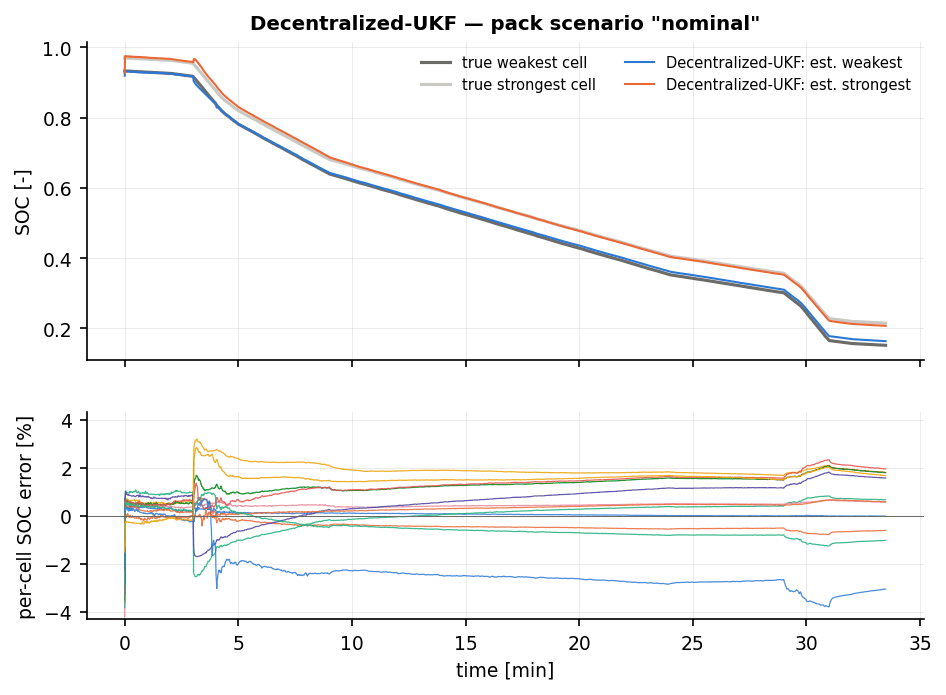
\includegraphics[width=\textwidth]{figures/pack_DecentralizedUKF_nominal.png}
\caption{Decentralized-UKF on the nominal eVTOL mission.}
\end{figure}
\begin{figure}[H]\centering
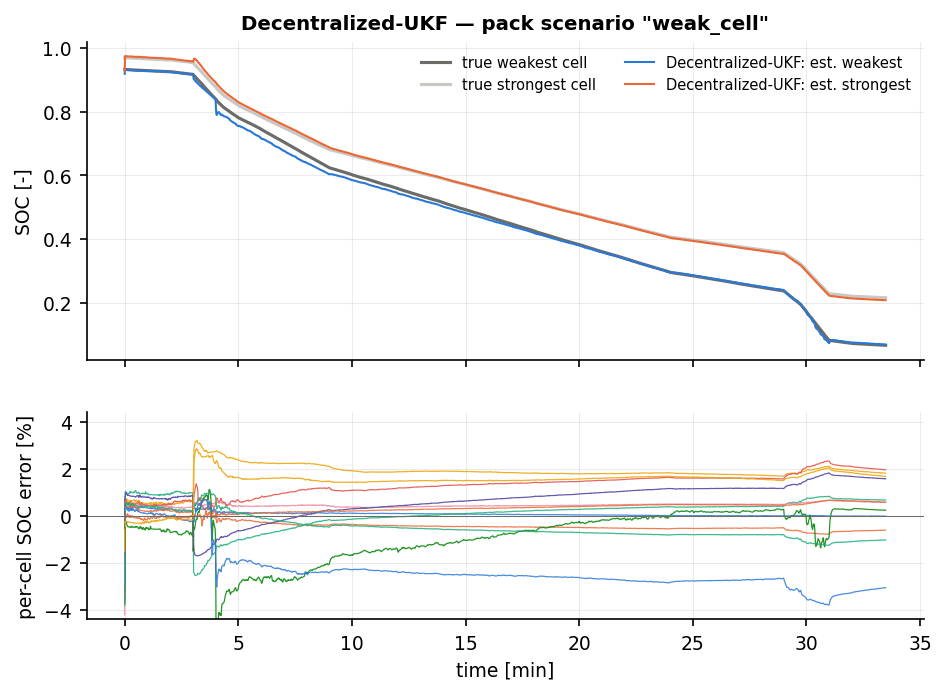
\includegraphics[width=\textwidth]{figures/pack_DecentralizedUKF_weak_cell.png}
\caption{Decentralized-UKF on \texttt{weak\_cell}: the weakest-cell SOC is the metric on which
this variant is furthest from the rest of the family.}
\end{figure}

Means over three seeds, against the EKF version of the same architecture:
\begin{center}\small
\begin{tabular}{@{}lcccc|cccc@{}}
\toprule
& \multicolumn{4}{c|}{\estname{Decentralized-UKF}} & \multicolumn{4}{c}{\estname{Decentralized-EKF}} \\
Scenario & rmse & rmse$_{\min}$ & ss & max & rmse & rmse$_{\min}$ & ss & max \\
\midrule
\texttt{nominal}          & 0.0141 & 0.0125 & 0.0143 & 0.057 & 0.0123 & 0.0081 & 0.0134 & 0.046 \\
\texttt{init\_error}      & 0.0167 & 0.0193 & 0.0159 & 0.065 & 0.0118 & 0.0082 & 0.0129 & 0.042 \\
\texttt{current\_bias}    & 0.0150 & 0.0072 & 0.0153 & 0.060 & 0.0137 & 0.0088 & 0.0148 & 0.056 \\
\texttt{weak\_cell}       & 0.0234 & 0.0565 & 0.0199 & 0.130 & 0.0129 & 0.0129 & 0.0137 & 0.048 \\
\texttt{noise\_step}      & 0.0142 & 0.0126 & 0.0144 & 0.057 & 0.0122 & 0.0084 & 0.0131 & 0.045 \\
\texttt{large\_imbalance} & 0.0190 & 0.0180 & 0.0195 & 0.071 & 0.0174 & 0.0245 & 0.0179 & 0.061 \\
\midrule
\si{\nano\second}/step & \multicolumn{4}{c|}{11900} & \multicolumn{4}{c}{3860} \\
bytes & \multicolumn{4}{c|}{57120} & \multicolumn{4}{c}{52032} \\
\bottomrule
\end{tabular}
\end{center}

\paragraph{The cell filter is not the bottleneck.} The UKF is \SIrange{10}{20}{\percent}
\emph{worse} than the EKF on four of six scenarios and \num{3.0} times more expensive, while
every common-state architecture in this family is \SIrange{45}{55}{\percent} better than the EKF
at between $1/7$ and $1.6$ times its cost. The conclusion for a pack BMS is that the per-cell
error on this plant is dominated by parameter mismatch and by the information thrown away in
Assumption~\ref{as:dek-nocross}, not by the linearisation of $h$: at the operating point of the
eVTOL mission ($\soc$ between \num{0.95} and \num{0.20}) the OCV curve is mild enough that
$\ocv'$ is an adequate description over one prior standard deviation.

\paragraph{Where the sigma-point filter actually loses.} The two worst rows are
\texttt{weak\_cell} (\texttt{rmse}$_{\min}=\num{0.0565}$ against \num{0.0129}) and
\texttt{init\_error} (\num{0.0193} against \num{0.0082}), both of which involve a \emph{large}
prior: in the first case the weak cell drifts \num{0.10} away from the nominal trajectory used to
seed the sigma points, in the second the prior starts \SI{35}{\percent} off. With a large
$\mP$ the subtractive covariance update of \eqref{eq:duk-ut} loses more accuracy than the
Joseph-form EKF update, and \texttt{cholesky\_safe} then has to jitter the factorisation. It does
not diverge --- \texttt{diverged} is zero in all eighteen runs --- but the worst single-cell
error reaches \num{0.130}, the largest in the family after the reduced-order model.

\paragraph{Where it wins.} \texttt{current\_bias}, on the weakest-cell metric
(\texttt{rmse}$_{\min}=\num{0.0072}$ against \num{0.0088}): the second-order correction of the
unscented transform partially compensates the systematic overpotential error that a current bias
produces, an effect that also appears in the cell-level chapters.

\section{Summary}
Decentralized-UKF is the control experiment of this family. It shows that on a 12-cell series
module with a 2-RC ESC model, improving the \emph{cell} filter beyond a Joseph-form EKF buys
nothing, while changing the \emph{pack} architecture halves the error. Use a sigma-point cell
filter when the per-cell nonlinearity really is the limiting factor --- LFP chemistry with its
flat OCV plateau, or operation below \SI{10}{\percent} SOC --- and combine it with a common-state
architecture rather than with a decentralised one; \texttt{BarDeltaPack} and
\texttt{FederatedPack} are both templates over the cell filter and accept \texttt{Ukf} directly.
